\documentclass{exam}
\usepackage[utf8]{inputenc}
\usepackage{lmodern}
\usepackage{microtype}

% \usepackage[parfill]{parskip}
\usepackage[dvipsnames]{xcolor}
\usepackage{amsmath}
\usepackage{amsfonts}
\usepackage{amsthm}
\usepackage{siunitx}
\DeclareSIUnit\year{yr}
\DeclareSIUnit\foot{ft}
\DeclareSIUnit\litre{\liter}

\usepackage{skull}

\usepackage{pgfplots}
\usepgfplotslibrary{polar}
\pgfplotsset{compat=1.11}
\usepgfplotslibrary{statistics}
\usepackage{graphicx}
\usepackage{sidecap}
\sidecaptionvpos{figure}{c}
\usepackage{float}
\usepackage{gensymb}
\usepackage{tkz-euclide}
\usetkzobj{all}
\usepackage{commath}
\usepackage{hyperref}
\usepackage{enumitem}
\usepackage{wasysym}
\usepackage{multicol}
\usepackage{mathtools}
\usepackage{tcolorbox}
\usepackage{tabularx}
\usepackage[version=4]{mhchem}
\usepackage{changepage}
\usepackage{listings}
\lstset{basicstyle=\ttfamily\linespread{0.8}\small}

\renewcommand*{\thefootnote}{\fnsymbol{footnote}}

\newtheorem*{thm}{Theorem}
\newtheorem*{iden}{Identity}
\newtheorem*{lemma}{Lemma}
\newtheorem{obs}{Observation}
\theoremstyle{definition}
\newtheorem*{defn}{Definition}
\newtheorem*{ex}{Example}
\newtheorem{con}{Construction}
\newtheorem*{alg}{Algorithm}

\newtheoremstyle{break}
  {\topsep}{\topsep}%
  {\itshape}{}%
  {\bfseries}{}%
  {\newline}{}%
\theoremstyle{break}
\newtheorem*{bthm}{Theorem}

% russian integral
\usepackage{scalerel}
\DeclareMathOperator*{\rint}{\scalerel*{\rotatebox{17}{$\!\int\!$}}{\int}}

% \DeclareMathOperator*{\rint}{\int}

\pgfplotsset{vasymptote/.style={
    before end axis/.append code={
        \draw[densely dashed] ({rel axis cs:0,0} -| {axis cs:#1,0})
        -- ({rel axis cs:0,1} -| {axis cs:#1,0});
    }
}}

% \pointsinrightmargin
\boxedpoints
\pointname{}

\newcommand{\questioA}{\question[\texttt{\textbf{\color{Cerulean} A}}]}
\newcommand{\questioM}{\question[\texttt{\textbf{\color{PineGreen} M}}]}
\newcommand{\questioE}{\question[\texttt{\textbf{\color{WildStrawberry} E}}]}
\newcommand{\questioS}{\question[\texttt{\textbf{\color{Goldenrod} S}}]}
\newcommand{\questioO}{\question[\texttt{\textbf{\color{BurntOrange} O}}]}

\newcommand{\parA}{\part[\texttt{\textbf{\color{Cerulean} A}}]}
\newcommand{\parM}{\part[\texttt{\textbf{\color{PineGreen} M}}]}
\newcommand{\parE}{\part[\texttt{\textbf{\color{WildStrawberry} E}}]}
\newcommand{\parS}{\part[\texttt{\textbf{\color{Goldenrod} S}}]}
\newcommand{\parO}{\part[\texttt{\textbf{\color{BurntOrange} O}}]}

\newcommand{\subparA}{\subpart[\texttt{\textbf{\color{Cerulean} A}}]}
\newcommand{\subparM}{\subpart[\texttt{\textbf{\color{PineGreen} M}}]}
\newcommand{\subparE}{\subpart[\texttt{\textbf{\color{WildStrawberry} E}}]}
\newcommand{\subparS}{\subpart[\texttt{\textbf{\color{Goldenrod} S}}]}
\newcommand{\subparO}{\subpart[\texttt{\textbf{\color{BurntOrange} O}}]}

\newcommand{\mainHeader}[2]{\section*{NCEA Level 2 Mathematics\\#1. #2}}
\newcommand{\mainHeaderHw}[2]{\section*{NCEA Level 2 Mathematics (Homework)\\#1. #2}}
\newcommand{\seealso}[1]{\begin{center}\emph{See also #1.}\end{center}}
\newcommand{\drills}[1]{\begin{center}\emph{Drill problems: #1.}\end{center}}
\newcommand{\basedon}[1]{\begin{center}\emph{Notes largely based on #1.}\end{center}}

\begin{document}

\mainHeaderDiff{6}{Tangent and Normal Lines}
For the next few weeks, we will be studying the geometry and shape of functions using calculus. We begin in
this section by taking a look at how closely functions can be approximated by straight lines around a point.

\subsection*{Tangent Lines}
The \textbf{tangent line} of a function at a point is the unique line passing through that point such that the
line has the same slope as the function at that point. Because we actually ended up defining slope based
on the derivative, it follows that the equation of the tangent line to a curve at a point can be defined
using the derivative.

More formally, if we have some function $ f $ which is differentiable at a point $ (x_0, y_0) $ then the
tangent line to the function at that point has the equation
\begin{displaymath}
  (y - y_0) = f'(x_0) (x - x_0).
\end{displaymath}

\begin{ex}
  Consider the function $ y = \sin \tan x $. The derivative of this function is $ y' = \sec^2 x \cos \tan x $;
  at the point $ P(\frac{3\pi}{8}, 0.6649) $, the slope is $ -5.1 $.
  \begin{center}
    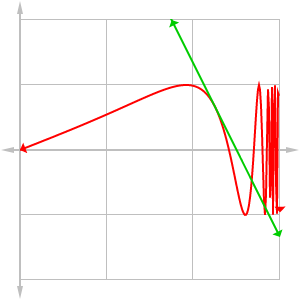
\includegraphics[width=0.35\textwidth]{tangentex}
  \end{center}

  The tangent line at $ P $ is $ y = \sin(\sqrt{2} + 1) + \cos(\sqrt{2} + 1)((\sqrt{2} + 1)^2 + 1)(x - \frac{3\pi}{8}) $, or
  (approximately) $ y = -5.1(x - 1.178) + 0.6649 $.
\end{ex}

The tangent line of a function at a point is the best linear approximation to the function at that point. This
means that if you know the value of a function and the derivative of that function at a point, then you can very
easily approximate the other values of the function around that point: if $ y_0 = f(x_0) $, and $ x $ is very
close to $ x_0 $, then
\begin{displaymath}
f(x) \approx f'(x_0)(x - x_0) + y_0.
\end{displaymath}
On the other hand, as the graph accompanying the example above shows, the tangent line is an awful approximation as
we move further away from the point that we find the tangent line at. It is possible to obtain some measure of the
error of a given approximation; this is explored, a little, in the exercises.

\begin{ex}
  Let us calculate $ \sqrt{4.03} $ by hand(!). If we consider the function $ f(x) = \sqrt{4 + x} $,
  then $ \sqrt{4.03} = f(0.03) $. Let's draw the situation out:
  \begin{center}
    \begin{tikzpicture}
      \begin{axis}[
        axis lines = center,
        xlabel = $ x $,
        ylabel = {$ y $}
      ]
        \addplot[domain = -4:6, color = green, samples=100] {sqrt(4+x)};
        \draw (4.03,0) -- (4.03,4);
        \node[label=left:{$ x = 4.03 $}] at (4.1,1.5) {};
        \node[label=above:{$ y = \sqrt{4 + x} $}] at (-2.2, 1.6) {};
      \end{axis}
    \end{tikzpicture}
  \end{center}
  So we want the tangent line to $ f $ at the point $ x = 0 $. We have that $ f'(x) = \frac{1}{2\sqrt{4 + x}} $ ,
  and so $ f'(0) = \frac{1}{4} $. The tangent line is the line through $ (0, f(0)) = (0, 2) $ with gradient $ \frac{1}{4} $,
  which has equation
  \begin{displaymath}
    y - 2 = \frac{1}{4}x.
  \end{displaymath}
  Hence $ \sqrt{4.03} \approx \frac{1}{4} \times 0.03 + 2 = 2.0075 $ --- and, as promised, all of these calculations
  can be done without a calculator. (According to my calculator, $ \sqrt{4.03} \approx 2.007486 $ and so we are not far
  off at all.)

%   Let us now calculate the error of this approximation. The difference between the actual and approximate values of
%   the square root is $ \left(\frac{1}{4}x + 2\right) - \sqrt{4 + x} $; if we want our error to be less than $ E \% $
%   of the real value, then we must solve
%   \begin{displaymath}
%     \abs{\left(\frac{1}{4}x + 2\right) - \sqrt{4 + x}} < \frac{E}{100} \sqrt{4 + x}
%   \end{displaymath}
%   for $ x $. Luckily, this is basically a polynomial in $ u = \sqrt{4 + x} $; making this substitution, we have
%   \begin{gather*}
%     \left(\frac{u^2}{4} + 1 - u\right)^2 < \left(\frac{E}{100}\right)^2 u^2\\
%     \frac{u^4}{16} + 1 + u^2 + \frac{u^2}{2} - \frac{u^3}{2} - 2u < \left(\frac{E}{100}\right)^2 u^2\\
%     0 < -\frac{1}{16}u^4 + \frac{1}{2}u^3 + \left(\frac{E^2}{10000} - \frac{3}{2}\right)u^2 + 2u - 1
%   \end{gather*}
%   We can now use our calculator to find the roots of this polynomial (or, if you were so inclined, there are various
%   methods for finding an approximation by hand); for example, if $ E = 100 $ then $ 4 - 2\sqrt{2} < u < 4 + 2\sqrt{2} $
%   is the region within which our approximation is `good'.
\end{ex}

\subsection*{Normal Lines}
If a function has a tangent line at a particular point, then the line perpendicular to the tangent line
at that point is called the \textbf{normal line}.

\begin{thm}
  If a tangent line has slope $ m $, then the normal line to it has slope $ m^\perp = -1/m $.
\end{thm}

\begin{center}
  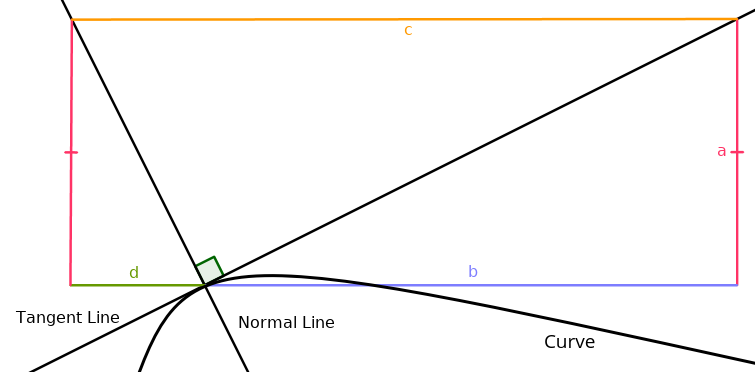
\includegraphics[width=0.6\textwidth]{normal-line-proof}
\end{center}

\begin{proof}
  Consider the line shown in the diagram above, and let $ m = \frac{a}{b} $ be the slope of the tangent line.
  So the length of the hypotenuse of the $ ab $ triangle is $ \sqrt{a^2 + b^2} $. But $ c = d + b $. Hence the length
  of the hypotenuse of the $ ad $ triangle can be found in two ways:
  \begin{displaymath}
    \sqrt{(d + b)^2 - \left(\sqrt{a^2 + b^2}\right)^2} = \sqrt{a^2 + d^2}.
  \end{displaymath}
  We can square both sides to obtain $ d^2 + 2db + b^2 - a^2 - b^2 = a^2 + d^2 $, and therefore $ db = a^2 $.
  Hence $ d/a = a/b $; but $ a/b = m $, and so the slope of the normal line is simply $ -\frac{a}{d} = -\frac{1}{m} $.
\end{proof}

\begin{ex}
  Consider the function $ f $ defined by $ f(x) = 2x^3 $. Then $ f'(x) = 6x^2 $, and the tangent line
  to the function at $ (2, 16) $ is $ (y - 16) = 24(x - 2) $, or $ y = 24x - 32 $. By the theorem above,
  the slope of the normal line to the function at that point is $ -1/24 $.

  \begin{center}
  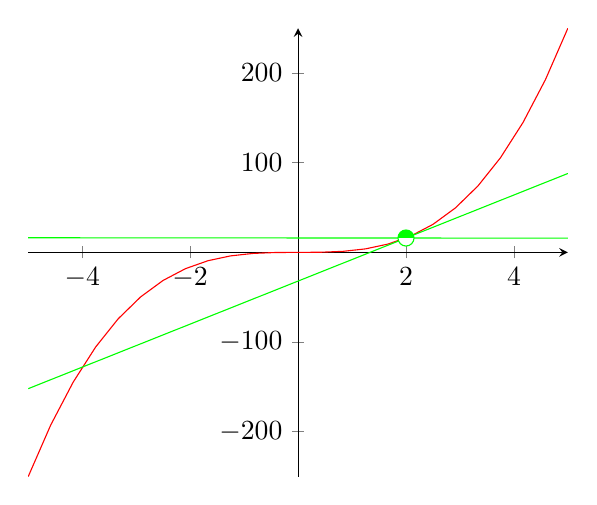
\begin{tikzpicture}
    \begin{axis}[axis lines=center]
      \addplot[color=red]{2*x^3};
      \addplot[color=green]{24*x - 32};
      \addplot[color=green]{(-1/24)*x + 1/12 + 16};
      \addplot[color=green, mark=halfcircle*, mark size=2.9pt]coordinates{(2,16)};
    \end{axis}
  \end{tikzpicture}
  \end{center}
\end{ex}

\clearpage
\subsection*{Questions}
\begin{questions}
  \questioA Draw the tangent and normal lines to each function at the indicated points.

    \begin{multicols}{2}
    \begin{parts}
      \part
        \begin{center}
        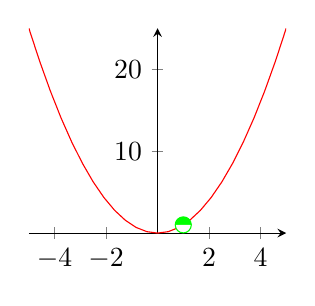
\begin{tikzpicture}
          \begin{axis}[axis lines=center, width=0.4\textwidth]
            \addplot[color=red]{x^2};
            \addplot[color=green, mark=halfcircle*, mark size=2.9pt]coordinates{(1,1)};
          \end{axis}
        \end{tikzpicture}
        \end{center}
      \part
        \begin{center}
        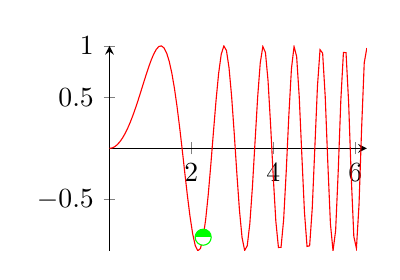
\begin{tikzpicture}
          \begin{axis}[axis lines=center, width=0.4\textwidth]
            \addplot[color=red, samples=100, domain=0:2*pi]{sin(deg(x^2))};
            \addplot[color=green, mark=halfcircle*, mark size=2.9pt]coordinates{(sqrt(5*pi/3),-0.86603)};
          \end{axis}
        \end{tikzpicture}
        \end{center}
      \part
        \begin{center}
        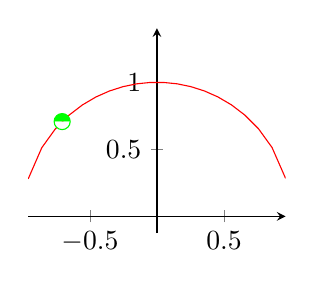
\begin{tikzpicture}
          \begin{axis}[axis lines=center, width=0.4\textwidth, axis equal]
            \addplot[color=red, samples=100]{sqrt(1-x^2)};
            \addplot[color=green, mark=halfcircle*, mark size=2.9pt]coordinates{(-0.707,0.707)};
          \end{axis}
        \end{tikzpicture}
        \end{center}
      \part
        \begin{center}
        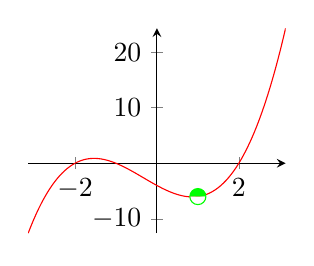
\begin{tikzpicture}
          \begin{axis}[axis lines=center, width=0.4\textwidth]
            \addplot[color=red, samples=100, domain=-pi:pi]{(x+1)*(x+2)*(x-2)};
            \addplot[color=green, mark=halfcircle*, mark size=2.9pt]coordinates{(1,-6)};
          \end{axis}
        \end{tikzpicture}
        \end{center}
    \end{parts}
    \end{multicols}
  \questioM Find the tangent and normal lines to the following functions at the given points.
    \begin{parts}
      \part $ x \mapsto \sin x $ at $ (0, 0) $
      \part $ x \mapsto \sin x $ at $ (\pi, 0) $
      \part $ x \mapsto e^x $ at $ (0, 1) $
      \part $ x \mapsto \sec x $ at $ (0, 0) $
      \part $ x \mapsto x^2 $ at $ (1, 1) $
      \part $ x \mapsto \sqrt{x} $ at $ (1, 1) $
      \part $ x \mapsto (x^4 - 3x^2 + 5)^3 $ at $ (0, 125) $
      \part $ x \mapsto \cos \tan x $ at $ (\pi, 1) $
      \part $ x \mapsto \left( x + \frac{1}{x^2} \right)^{\sqrt{7}} $ at $ (1, 2^{\sqrt{7}}) $.
    \end{parts}
  \questioM Find the equation of the tangent line to $ y = x + \tan x $ at $ (\pi, \pi) $.
  \questioM Find an equation for the normal line to the curve $ y = \frac{1}{\sqrt{x^2 - x}} $ at $ (2, \frac{1}{\sqrt{2}}) $.
  \question Consider the curve $ y = \tan(2\sin x) $.
    \begin{parts}
      \parA Show that $ \od{y}{x} = 2\cos x \sec^2 (2 \sin x) $.
      \parM Find the equation of:
        \begin{subparts}
          \subpart The tangent to the curve at $ (\pi, 0) $
          \subpart The normal to the curve at $ (0, 0) $
        \end{subparts}
    \end{parts}
  \questioM Find the best linear approximation to $ y = 3x^3 + 2x + 4 $ around $ x = 2 $.
  \questioM Find the point(s) on the graph of the function $ y = x^2 $ such that the slope of the normal to the curve at that point is $ m^\perp = -1 $.
  \questioE The tangents to the curve $ y = \frac{1}{4}(x - 2)^2 $ at points $ P $ and $ Q = (6,4) $ are perpendicular. What is the $ x$-ordinate of $ P $?
  \questioS Consider the surface described by $ z = x^2 + 2\sin(y^2 + 1) + 2 $.
    \begin{parts}
      \part Find the derivative of $ z $ with respect to $ x $, and find the tangent line in the $ x $ direction at $ (0,0) $.
      \part Find the derivative of $ z $ with respect to $ y $, and find the tangent line in the $ y $ direction at $ (0,0) $.
      \part Hence describe the tangent \textit{plane} of the surface at $ (0,0) $.
    \end{parts}
  \question Consider the function $ y = \sin x $.
    \begin{parts}
      \parM Find the best linear approximation to this function around $ (0,0) $.
      \parM Find the percentage error of this approximation to 1dp when $ x = \pi $.
      \parE At what point on the curve ($ x \geq 0 $) does the percentage error of the approximation rise above $ 100\% $?
    \end{parts}
  \question
    \begin{parts}
      \parM Find two points on the graph of $ y = 1/x $ that share a common normal line.
      \parM Show that there are no more such points.
      \parM Show that there are no two points on the graph that share a common tangent line.
      \parE Repeat parts (a)-(c) for the general hyperbola-like curve $ y = x^{-n} $ (where $ n $ is a positive integer).
      \parS What is the situation for the even more general case of the curve $ y = x^r $, where $ r $ is any real number?
    \end{parts}
  \question Consider the quartic polynomial $ p(x) = 2x^4 -4x^3 - 23x^2 + 84x - 61 $.
    \begin{parts}
      \parM Find the best linear approximation to $ p $ around the point $ (2, 15) $.
      \parS Find the unique quadratic polynomial $ q(x) $ such that $ q(2) = p(2) $, $ q'(2) = p'(2) $, and $ q''(2) = p''(2) $.
            This is the best quadratic approximation to $ p $ at the point $ (2, 15) $.
      \parO Show that the best quadratic approximation to a function $ f $ at the point $ (x_0, y_0) $ is given by
            \begin{displaymath}
              T_2(x) = f(x_0) + f'(x_0) (x - x_0) + \frac{1}{2} f''(x_0) (x - x_0)^2.
            \end{displaymath}
    \end{parts}
\end{questions}
\end{document}
